\section{Data Check}\label{sec:datacheck}

\textbf{Kirchhoff check.} Because the currents are recorded into the terminals, $i_d+i_g+i_s+i_b$ must vanish. Table~\ref{tab:kcl} gives the residual for every case: the median is at most $\num{1.14e-6}$ of the largest terminal current (the six-digit CSV precision and \texttt{reltol}$=10^{-6}$; $\num{4.85e-9}$ for PMOS ON) and the 95th percentile is below $\num{5.6e-6}$ in all four cases. The only larger residuals are 15 NMOS ON and 18 PMOS ON rows with a relative residual above $10^{-3}$ (maximum $\num{2.84e-2}$ and $\num{1.36e-2}$); all are barely-on devices whose largest terminal current is at most $\SI{1.4e-13}{\ampere}$, with an absolute residual of at most $\SI{7.7e-16}{\ampere}$, about three times the $\num{2.2e-16}$\,A resolution of the branch-current readout.
% src: partA_transistor/data_check/kcl_check.csv, partA_transistor/data_check/README.md
\begin{table}[t]
\caption{Kirchhoff check of the four datasets (relative = divided by the largest terminal current of the row).}
\label{tab:kcl}
\centering\footnotesize
\setlength{\tabcolsep}{2.5pt}
\fitcol{% src: partA_transistor/data_check/kcl_check.csv
\begin{tabular}{lrrrrr}
\toprule
Case & Median $|\Sigma I|$ (A) & Max $|\Sigma I|$ (A) & Median rel. & P95 rel. & Max rel. \\
\midrule
NMOS ON & \num{8.18e-12} & \num{9.87e-10} & \num{5.1e-07} & \num{4.2e-06} & \num{2.8e-02} \\
NMOS OFF & \num{2.59e-17} & \num{8.29e-13} & \num{8.5e-07} & \num{3.9e-06} & \num{9.0e-06} \\
PMOS ON & \num{4.20e-14} & \num{1.00e-10} & \num{4.8e-09} & \num{1.6e-06} & \num{1.4e-02} \\
PMOS OFF & \num{1.00e-19} & \num{9.16e-13} & \num{1.1e-06} & \num{5.5e-06} & \num{9.9e-06} \\
\bottomrule
\end{tabular}
}
\end{table}

\textbf{Trend plots.} Figures~\ref{fig:trend1} and~\ref{fig:trend2} show the OFF current $\max(|i_d|,|i_s|)$ against temperature and against the threshold voltage, and the gate current $|i_g|$ against the oxide thickness, on log axes with the binned median. (Drain and source swap roles when $V_s>V_d$, so the larger of $|i_d|$ and $|i_s|$ is the channel leakage in either orientation.) All three trends have the expected sign in every case: the OFF current rises with temperature and falls with the threshold voltage, and the gate current falls steeply with the oxide thickness, by a factor of 20 to 170 over the 0.945--1.155\,nm range.
Over all rows the temperature and $V_{th}$ trends are diluted, because the OFF current also contains junction and gate-induced-drain leakage that depend little on either (a floor near $10^{-14}$\,A for PMOS OFF in Fig.~\ref{fig:trend1}). Restricting to the subthreshold regime (source within 50\,mV of its rail, other terminal more than 0.5\,V away, about 500 rows per case) gives the textbook behaviour: $+0.90$ (NMOS) and $+0.81$ (PMOS) decades per 100\,$^\circ$C and $-0.55$ and $-0.59$ decades per 50\,mV of $V_{th}$, i.e.\ roughly 84--91\,mV per decade.
% src: partA_transistor/data_check/trend_numbers.csv, partA_transistor/data_check/README.md
\begin{figure*}[t]
\centering
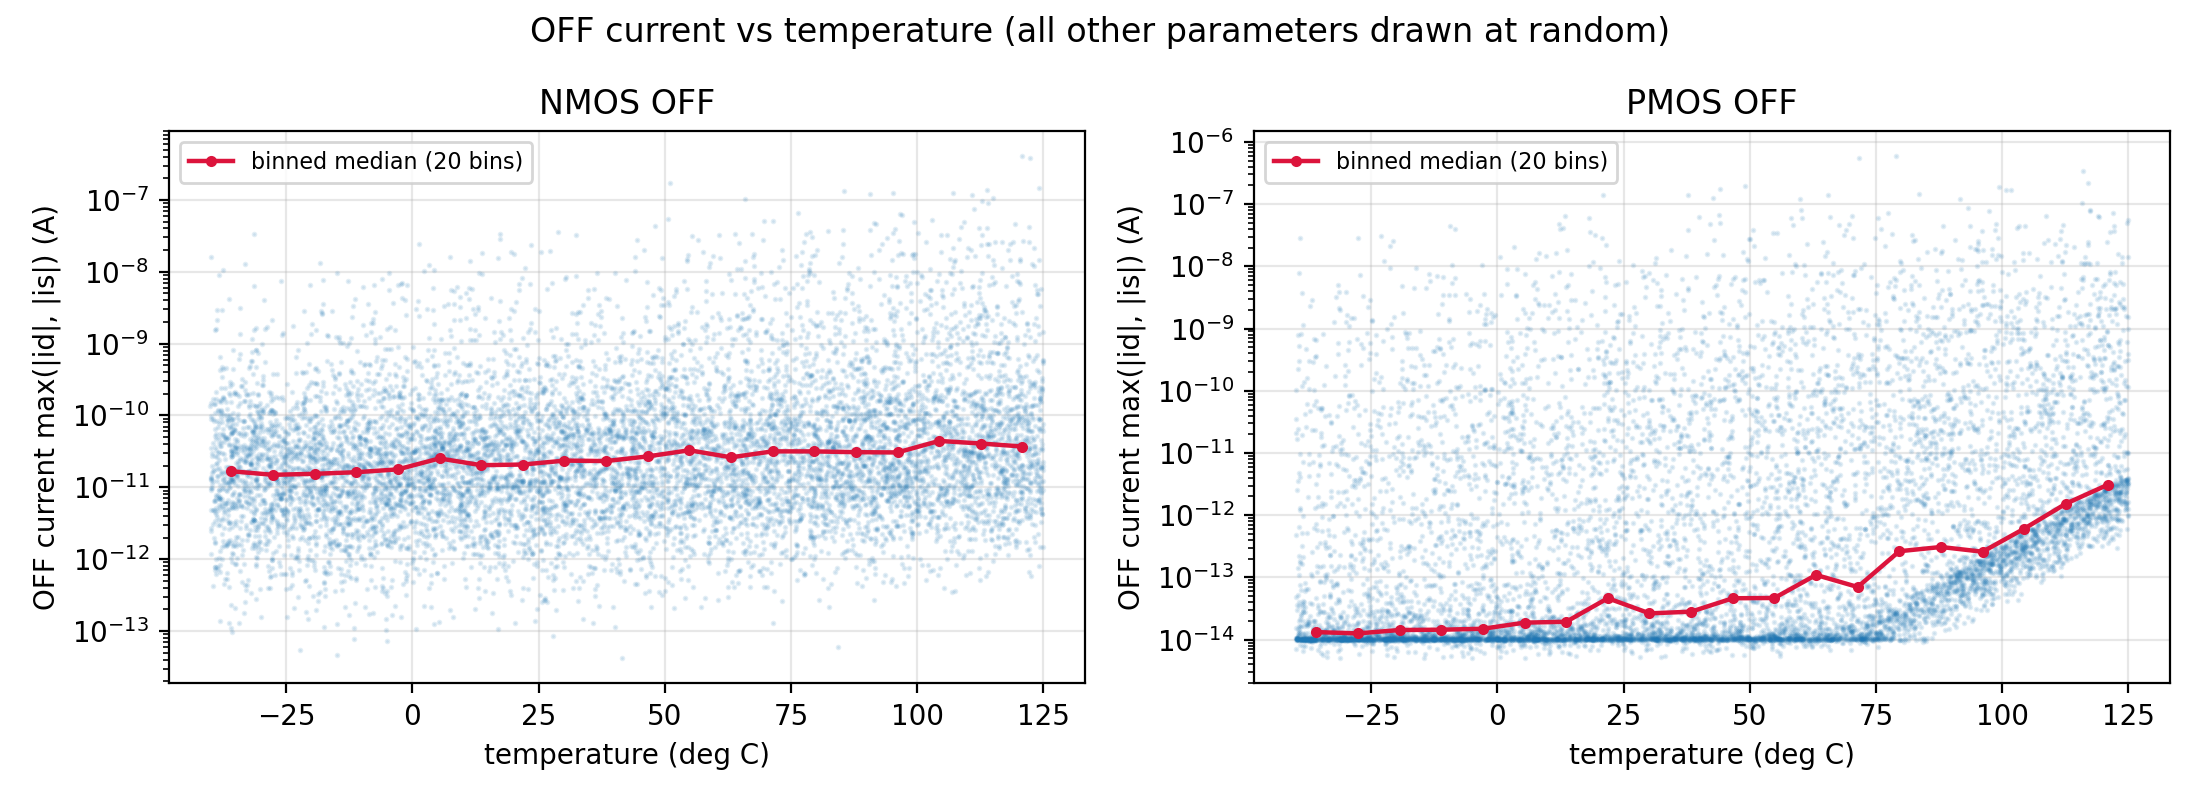
\includegraphics[width=0.49\textwidth]{figures/trend_off_vs_temperature.png}\hfill
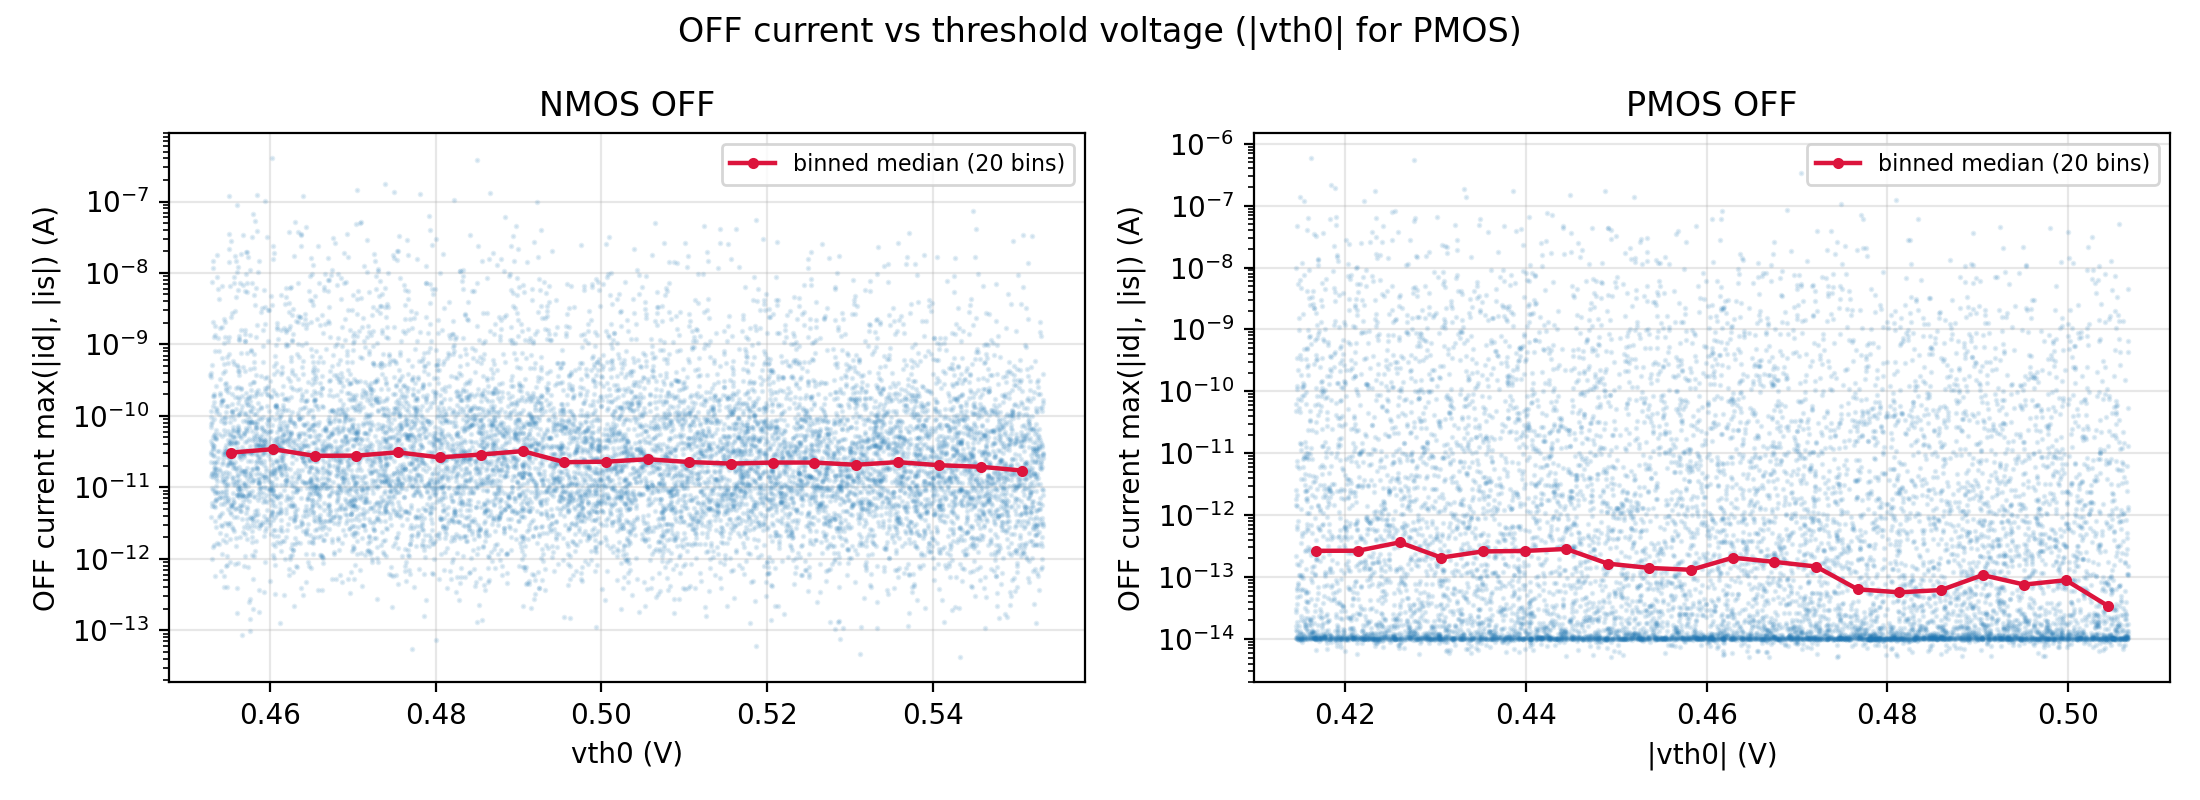
\includegraphics[width=0.49\textwidth]{figures/trend_off_vs_vth0.png}
\caption{OFF current $\max(|i_d|,|i_s|)$ versus temperature (left) and versus $|V_{th0}|$ (right) for NMOS OFF and PMOS OFF; faint points are the 10,000 samples, the red line is the median in 20 bins.}
\label{fig:trend1}
% src: partA_transistor/data_check/trend_off_vs_temperature.png, trend_off_vs_vth0.png
\end{figure*}
\begin{figure*}[t]
\centering
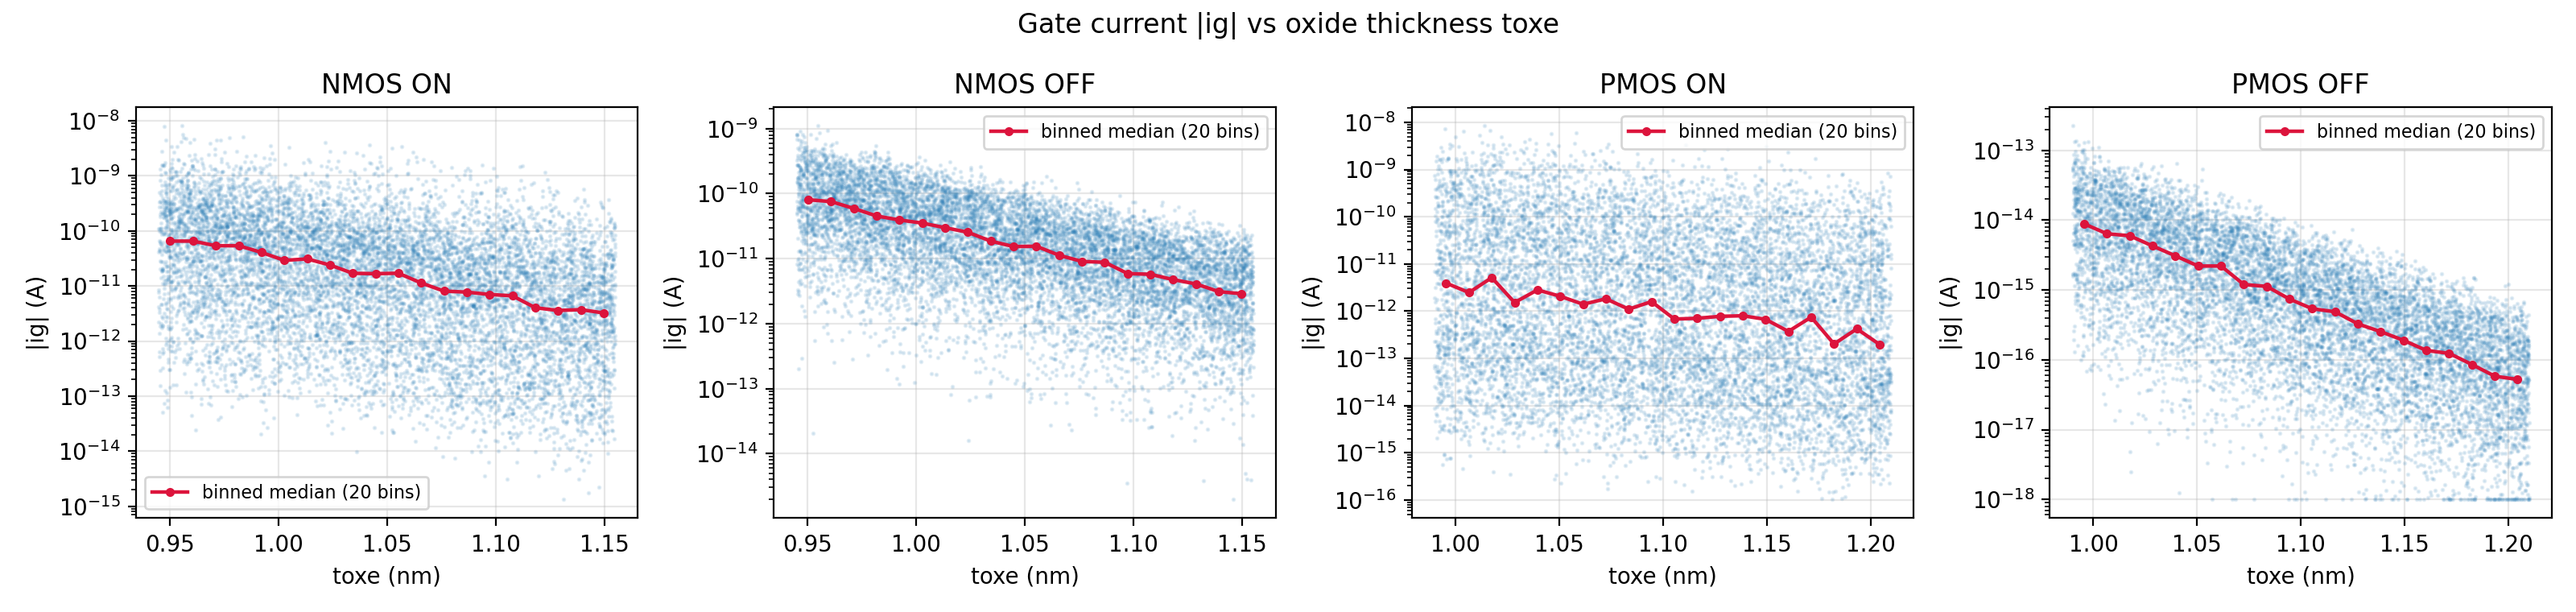
\includegraphics[width=0.9\textwidth]{figures/trend_ig_vs_toxe.png}
\caption{Gate current $|i_g|$ versus oxide thickness for all four cases (tunnelling current: steep fall of the median with toxe).}
\label{fig:trend2}
% src: partA_transistor/data_check/trend_ig_vs_toxe.png
\end{figure*}
